\section{Thrust distribution}

In order to validate the ALEPH archieved data sample and our understanding,
an analysis of the thrust distribution ($T$) is performed with LEP1 archieved
data. The distributions are corrected for the detector response by ALEPH MC
produced in 1994. The correction factors, which are obtained from ratio of generator level and detector level Thrust spectra, are shown in Figure~\ref{fig:ThrustCorr}. The size of the correction factor is small in the mid-$T$
and becomes larger as we go to smaller $T$ or larger $T$ regions.

\begin{figure}[H]
\centering
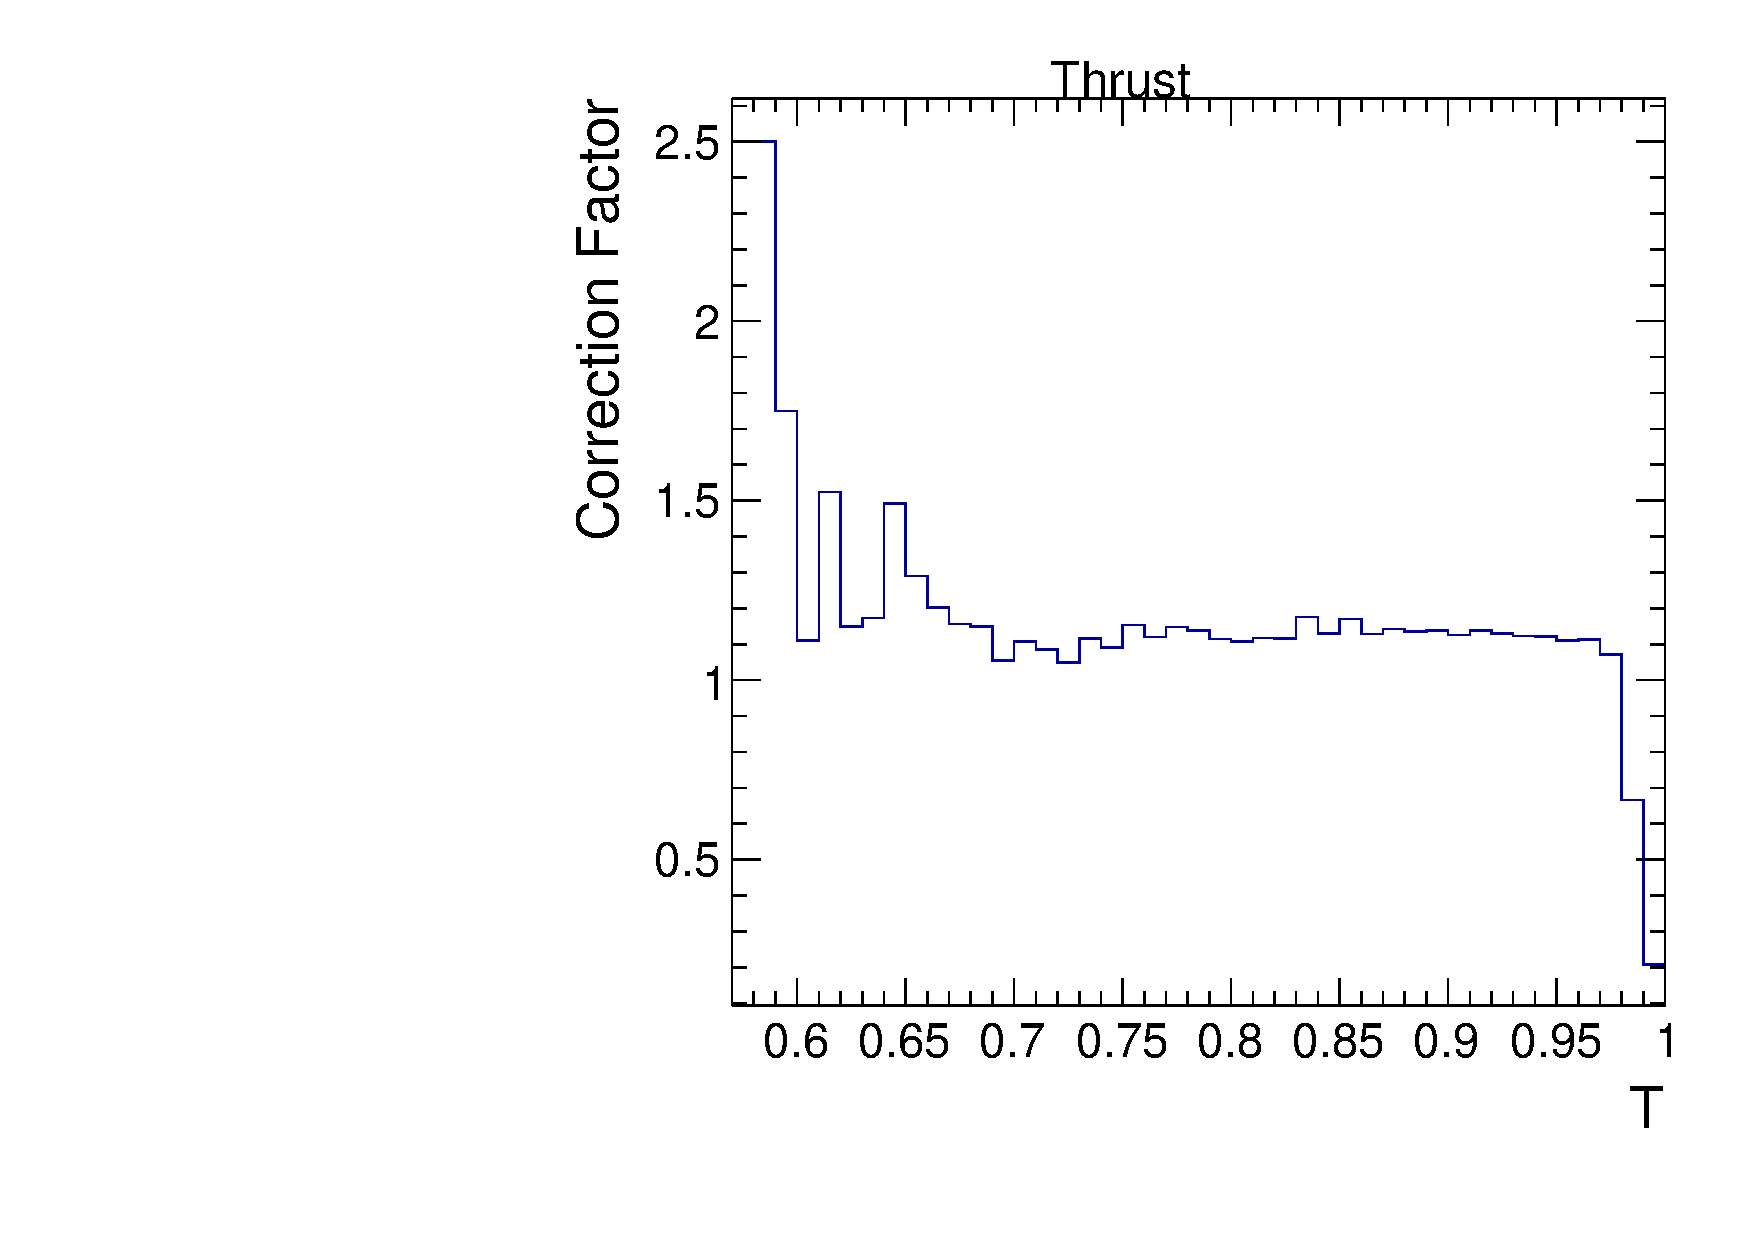
\includegraphics[width=.5\textwidth]{images/Thrust/correction.pdf}
\caption{The correction factor for the Thrust distribution measurement obtained from ALEPH MC.}
\label{fig:ThrustCorr}
\end{figure}

Figure~\ref{fig:ThrustResults} shows the corrected thrust distribution from ALEPH archieved data. The results are compared to ALEPH
publications~\cite{Barate:1996fi,heister:2003aj}. As shown in the figure, a very good agreement between ALEPH archieved data from this note
and ALEPH publications in the low $T$ region. In the $T\sim 1$ region, some disagreement at the level of 10\% is observed between this work
and the ALEPH publication in 2004~\cite{heister:2003aj}. This is probably due to the hadronzation correction which is not applied in
ref.~\cite{Barate:1996fi} and this work. 


\begin{figure}[H]
\centering
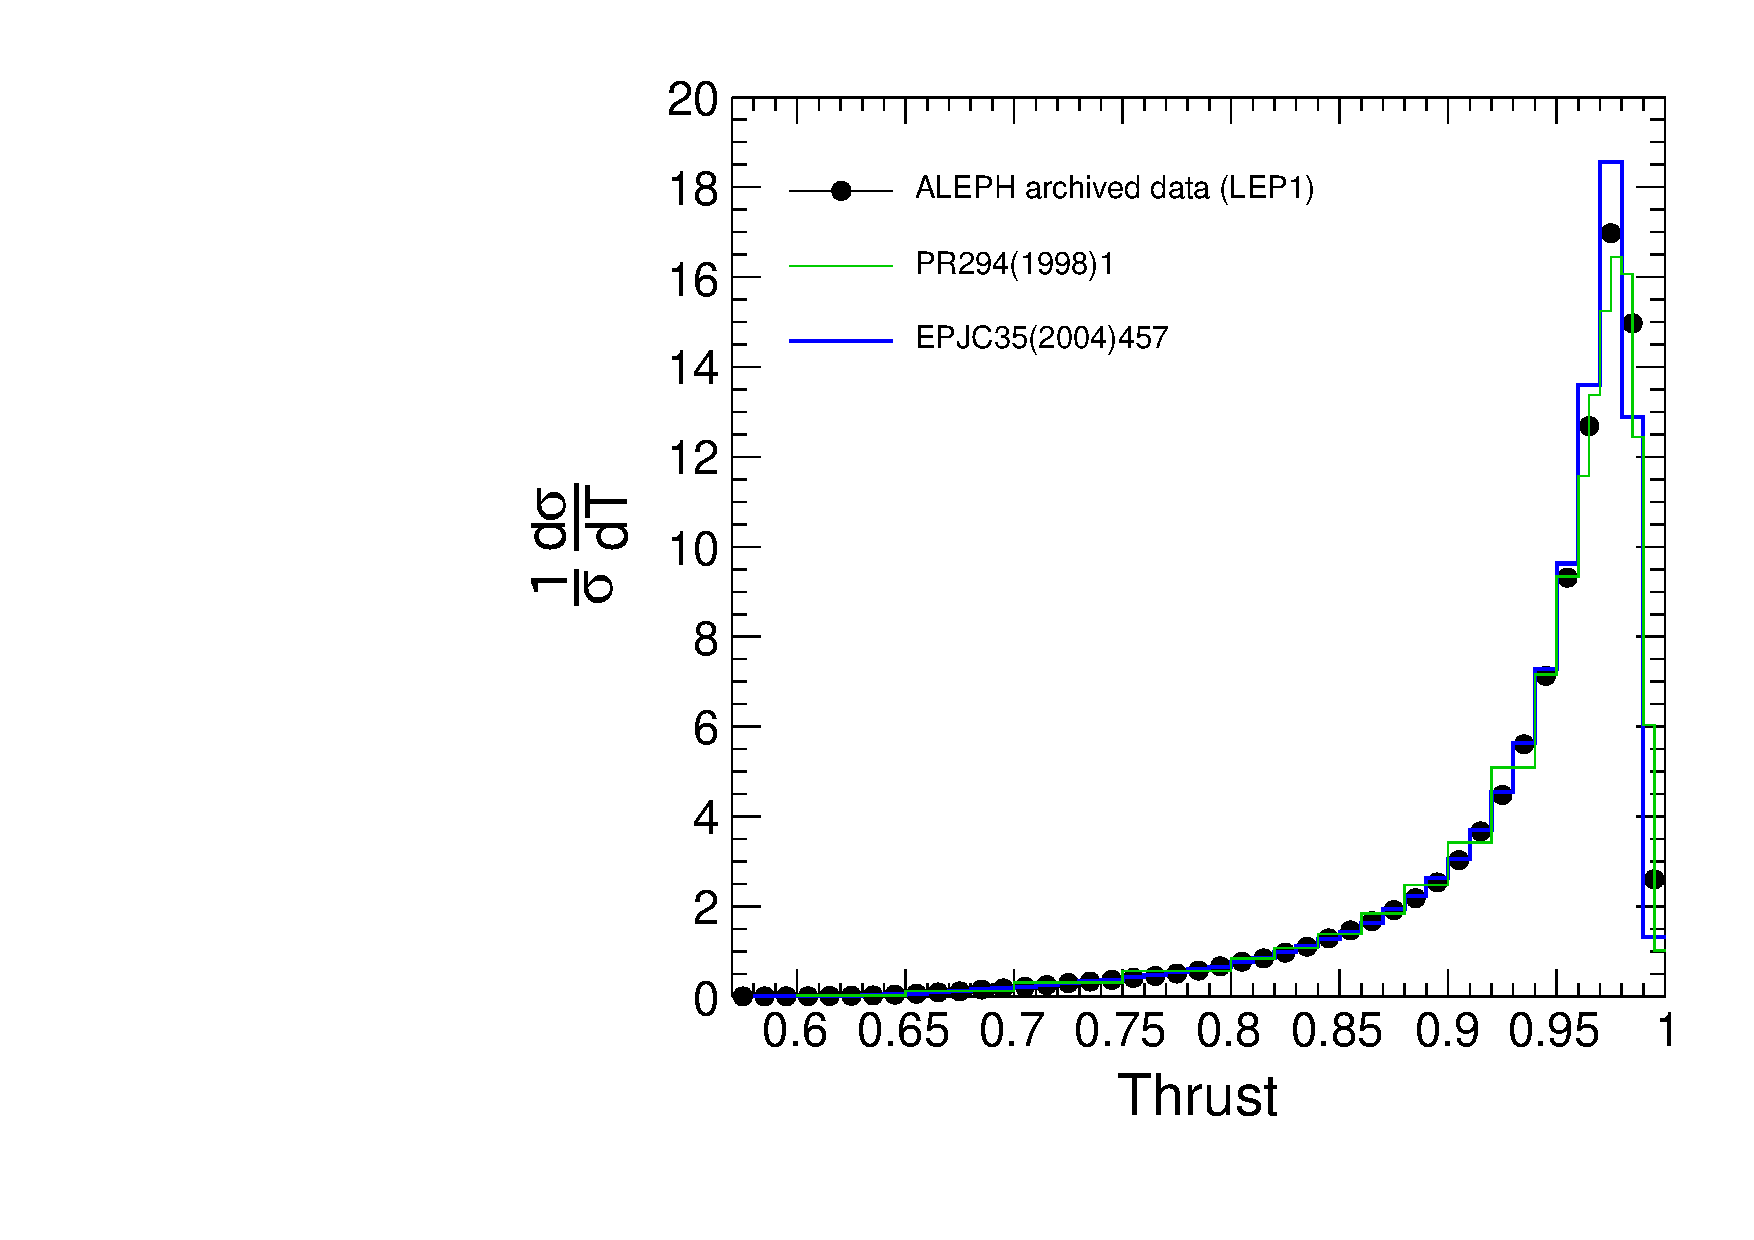
\includegraphics[width=.5\textwidth]{images/Thrust/mithig_T_LEP1_0_9999.pdf}
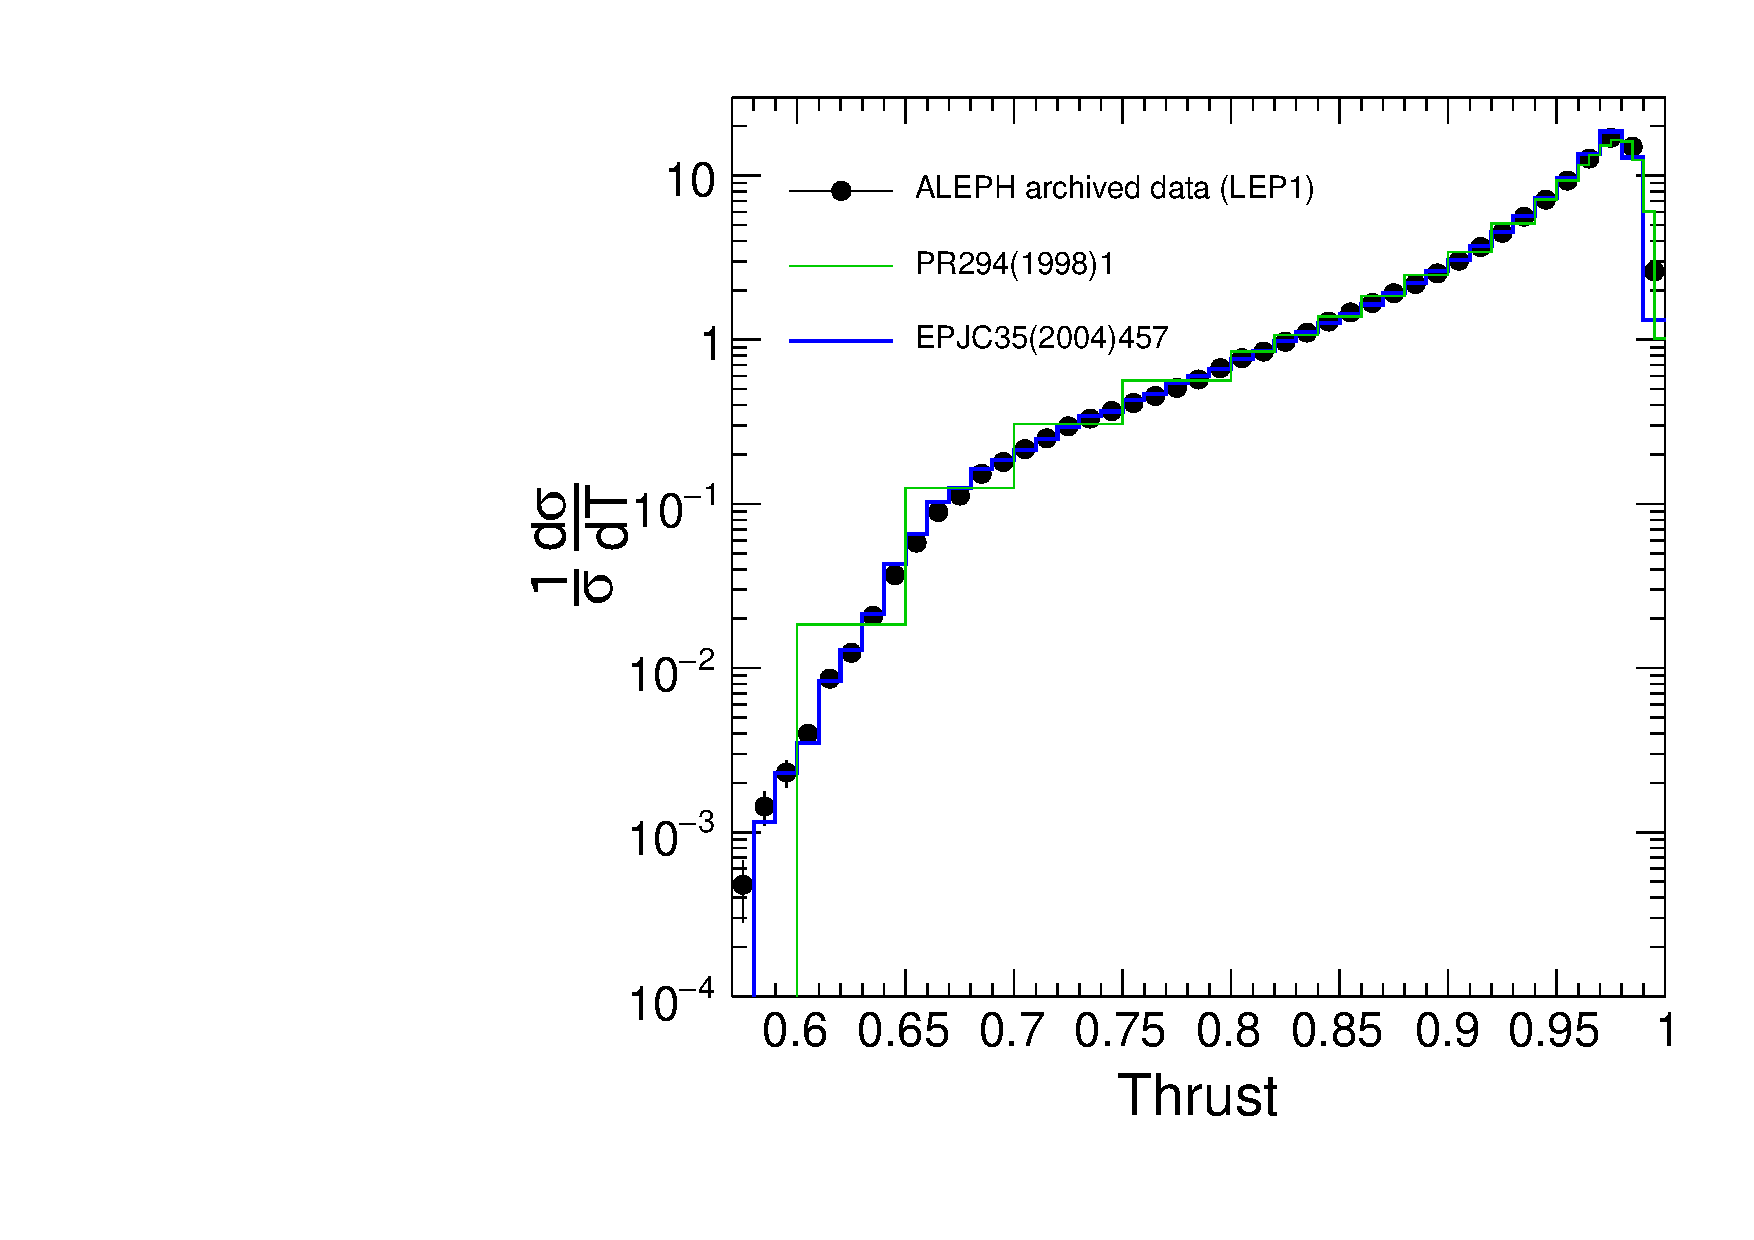
\includegraphics[width=.5\textwidth]{images/Thrust/mithig_T_log_LEP1_0_9999.pdf}
\caption{The corrected thrust distribution from ALEPH archieved data compared to previous pbulications in linear and log scale.}
\label{fig:ThrustResults}
\end{figure}
